%%%%%%%%%%%%%%%%%%%%%%%%%%%%%%%%%%%%%%%%%%%%%%%%%%%%%%%%
%GRASS PROMOTION FLYER                                 %
%(c) 2007 GRASS PROMOTION TEAM                         %
%GNU Free Documentation License                        %
%Version 1.2                                           %
%Needs leaflet.cls				       %
%www.ctan.org/tex-archive/macros/latex/contrib/leaflet/%
%%%%%%%%%%%%%%%%%%%%%%%%%%%%%%%%%%%%%%%%%%%%%%%%%%%%%%%%

%Sometimes printing engines need the 2nd side upside down
%in this case, use tumble (which is default) instead of notumble
%If this causes problems, use notumble
%If you need a foldmark, delete nofoldmark
\documentclass[notumble,a4paper,10pt,nofoldmark]{leaflet}
\usepackage{helvet,courier,xcolor}
\usepackage[utf8]{inputenc}

% Set Helvetica as the default font
\renewcommand*\familydefault\sfdefault
% Let LaTeX knows that pictures are found in ./pix
\graphicspath{{pix/}}

% Setting up things for the captions
\usepackage{caption}[2004/07/16]
\captionsetup{%
  font={small,it},%
  labelformat=empty,% Leaves out label: ``Figure 1''
  labelsep=none,%
  aboveskip=0pt%
}
% Defining a new 'figure' environment for the document
\newenvironment{myfig}[1][0pt plus 1.5ex minus .5ex]{\par\vspace*{#1}\begin{minipage}{\textwidth}\centering}{\end{minipage}}

% Defining the GRASS homepage
\newcommand{\GRASSurl}{\url{http://grass.itc.it}}

% Define a color for the URIs
\definecolor{darkblue}{RGB}{0,0,88}

\usepackage{hyperref}
% Setting up some document info
\hypersetup{%
  colorlinks=true,%
  urlcolor=darkblue,% Redefine this color to change URIs color
  pdfauthor={GRASS Community},%
  pdftitle={GRASS GIS: Učinnost Svodody \& Transparentnosti},%
  pdfsubject={GRASS propagační leták GRASS},%
  breaklinks=true,%
  plainpages=false%
}

% Title page stuff
\title{\textbf{\huge GRASS GIS}\\%
\textsl{Učinnost Svodody \& Transparentnosti}}
\author{Komunita GRASSu}
\date{
\includegraphics[width=\textwidth]{grasslogo_vector}\\[2ex]
\large\GRASSurl}

\begin{document}

\maketitle
\thispagestyle{empty}% Necessary to leave out the page number on the first page

\newpage

\section{Co je GRASS}

GRASS (Geographic Resources Analysis Support System) je svobodný/Open Source software určený pro prostorové analýzy. Obsahuje více než 350 modulů pro zpracování 2D/3D vektorových a rastrových dat. Nabízí řadu rozhraní k dalším programům v dané oblasti jako je geostatistika, databáze, mapové služby a dokonce i k dalším GIS aplikacím. Je nejrozsáhlejším Open Source GISem. Může sloužit jako Desktop GIS či jako páteř kompletní GIS infrastrukturu.

\section{Kde je GRASS používán}

GRASS je používán ve vědeckých aplikacích, komerčně či ve veřejné správě po celém světě. GRASS pokytuje v mnoha připadech velký potenciál pro řešení geoprostorových úloh.

\section{Historie}

GRASS byl původně vyvíjen od počátku 80-tých let agenturou US Army Construction Engineering Research Laboratories (USA-CERL) a byl poskytnut jako public domain software. V okamžiku kdy USA-CERL upustil od vývoje, vzniknul mezinárodní tým vývojářů který dál software vyvíjí. Od roku 1999 je GRASS uvolněn jako free software pod licencí GNU General Public Licence.
\begin{myfig}[1.5ex]
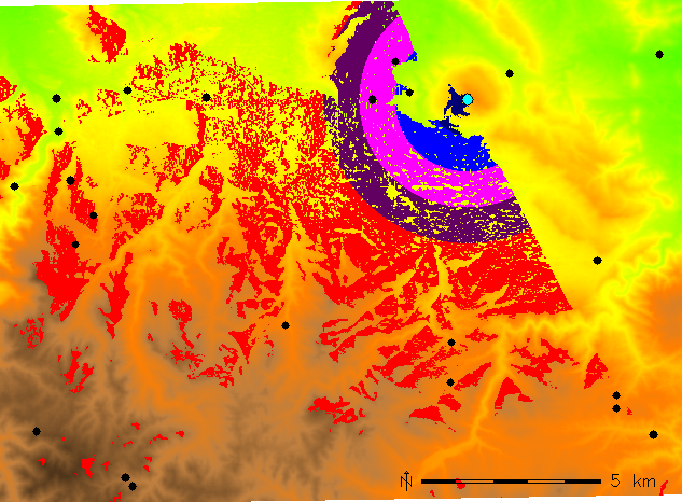
\includegraphics[width=0.7\textwidth]{visibility}
\captionof{figure}{Analýza viditelnost provedena v GRASSu}
\end{myfig}

\section{Filozofie Open Source}

Filozofie Open Source nabízí uživateli možnost nahlédnutí do zdrovových kódu a struktury programu, obrovskou míru transparentnosti. Uživatel může rozšířit program dle svých potřeb. Vzájemná kontrola zdrojového kódu zvyšuje jeho kvalitu. Tzv. extension manager umožňuje vytvářet nové moduly bez nutnosti zdrovového kódu GRASSu.

\section{Technická data}

\subsection{Licence}

Všeobecná veřejná licence GNU (GNU General Public License, Free Software Foundation)

\subsection{Podporované platformy}

GRASS běží na témeř všech platformách. Podporuje GNU/Linux, unixové systémy podporující Posix, MS-Windows a MacOS X.

\subsection{Design}

\begin{itemize}
\item Modulární
\item Obsahuje více než 350 modulů
\end{itemize}

\subsection{Programovací jazyky}

\begin{itemize}
\item ANSI C
\item Rozhraní GRASS- SWIG
\item Python pro WebGIS aplikace
\item Verze pro Javu: JGRASS
\end{itemize}

\subsection{Možnosti správy dat}

\begin{itemize}
\item Zpracování rasterových / vektorových / voxel dat
\item Modelování 2D / 3D rastrových / vektorových dat
\item Zpracování obrazových dat
\item Vektorová topologie / Síťové analýzy
\item Geostatistika (rozhraní pro R)
\end{itemize}

\begin{myfig}[1ex]
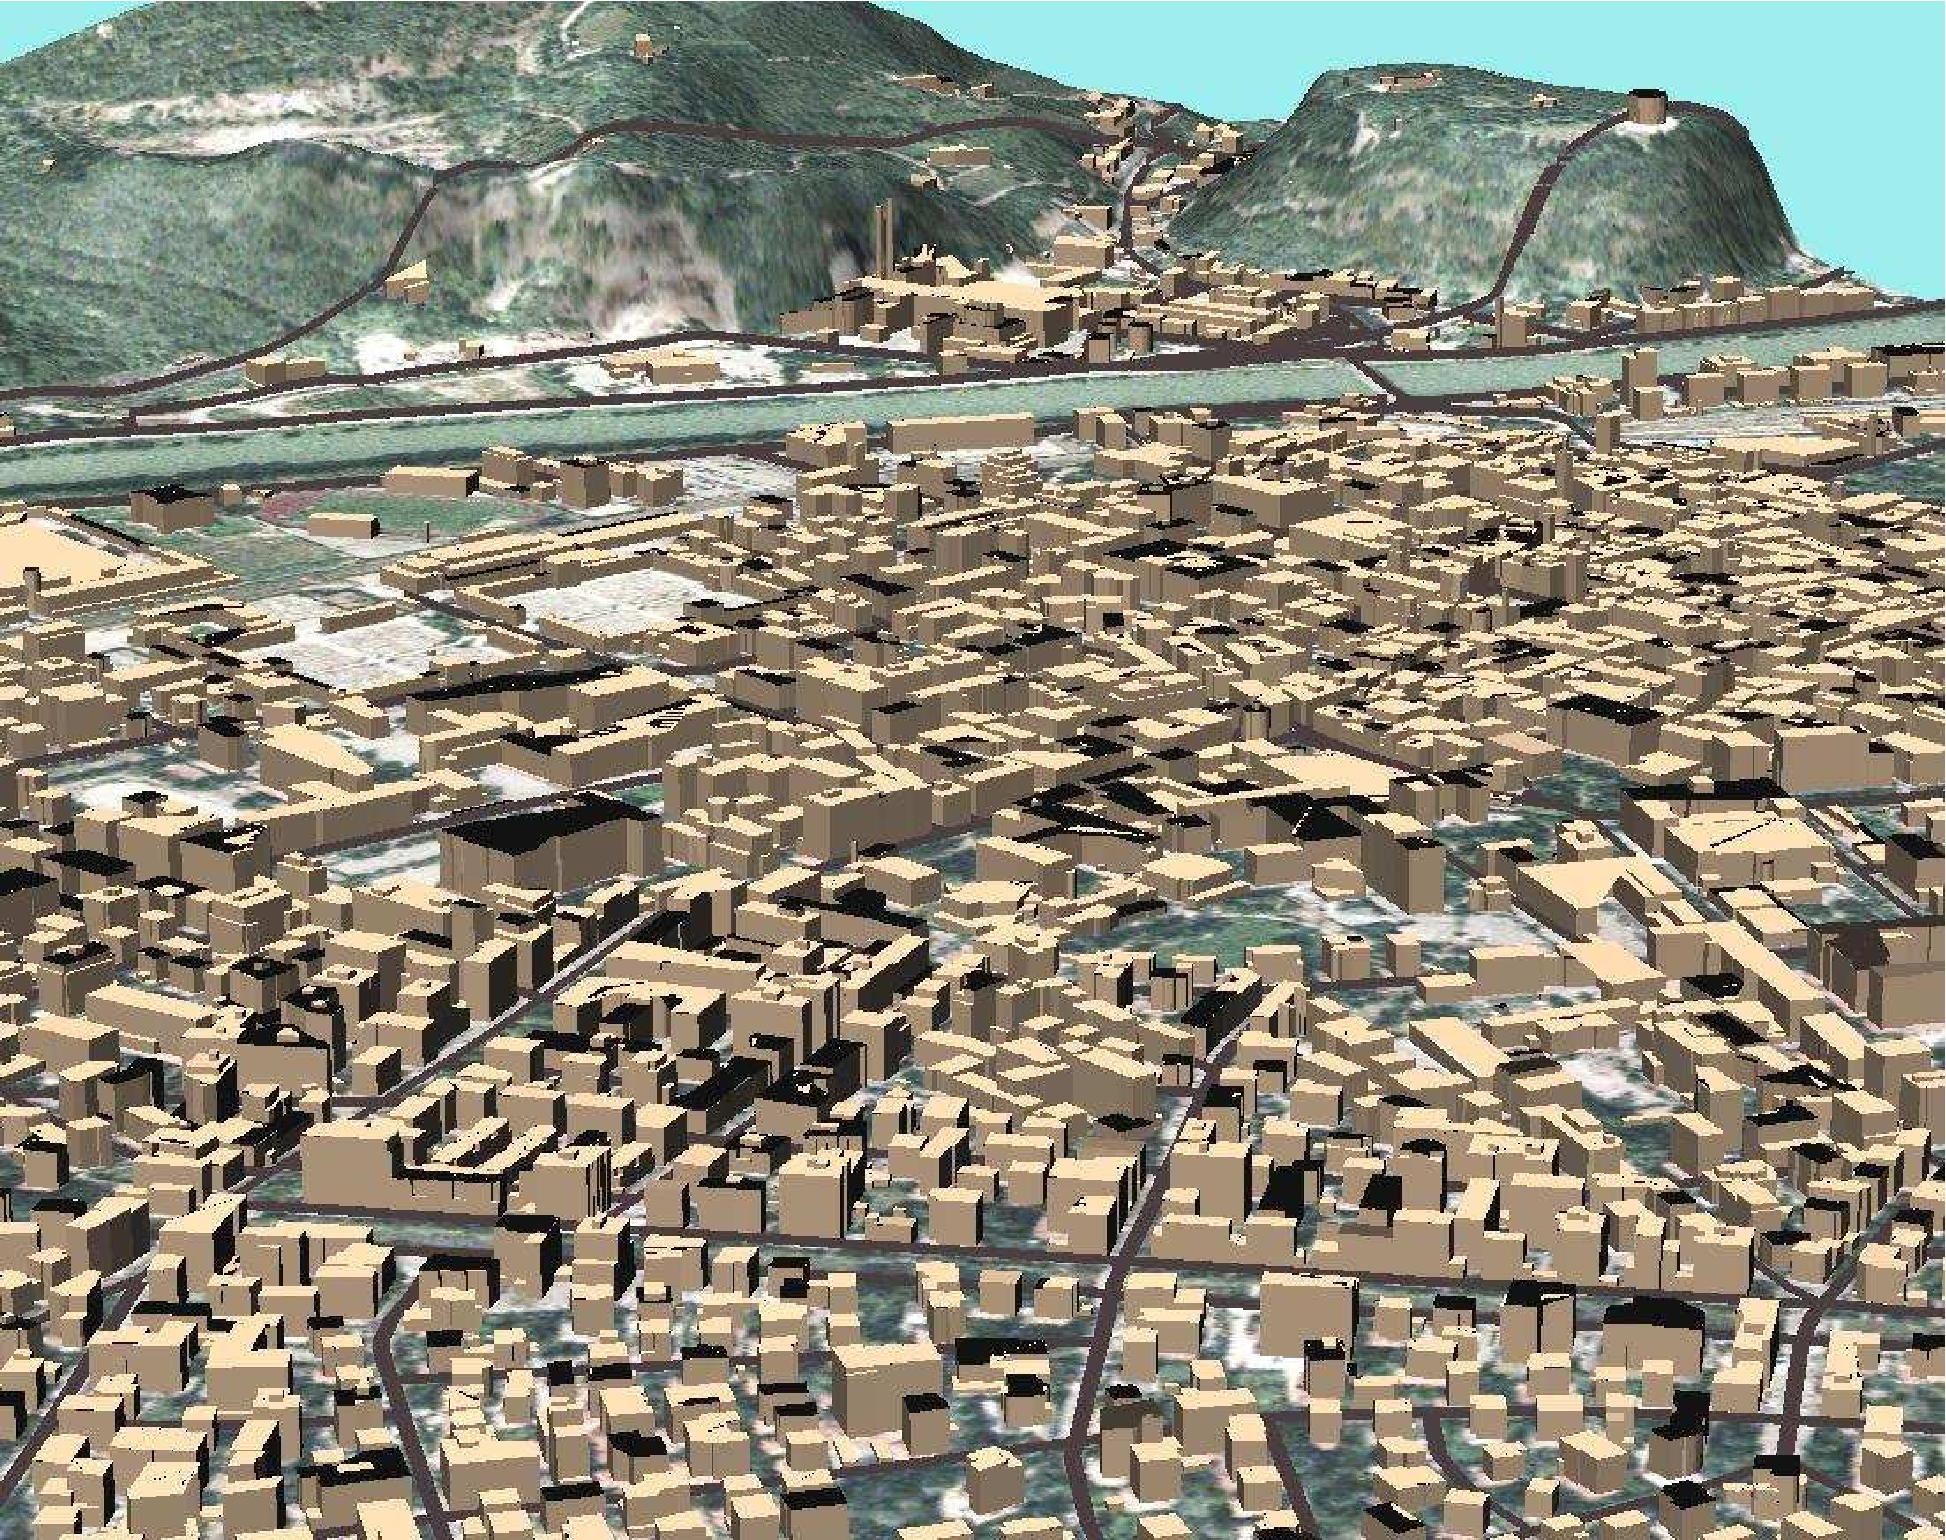
\includegraphics[width=0.7\textwidth]{trento3d}
\captionof{figure}{3D pohled na Trento, Itálie}
\end{myfig}

\section{Podporované datové formáty}

GRASS podporuje téměř všechny dobře známé GIS datové formáty díky knihovně GDAL/OGR. Navíc podporuje Open GIS Consortium's Simple Features.

\subsection{Vektorové datové formáty}
ASCII, ARC/INFO ungenerate, ARC/INFO E00, Arc\-View SHAPE, BIL, DLG (U.S.), DXF, DXF3D, GMT, GPS-ASCII USGS-DEM, IDRISI, MOSS, MapInfo MIF, TIGER, VRML, \dots

\subsection{Rastrové datové formáty}
ASCII, ARC/GRID, E00, GIF, GMT, TIF, PNG, Vis5D, SURFER (.grd),\dots
\begin{myfig}
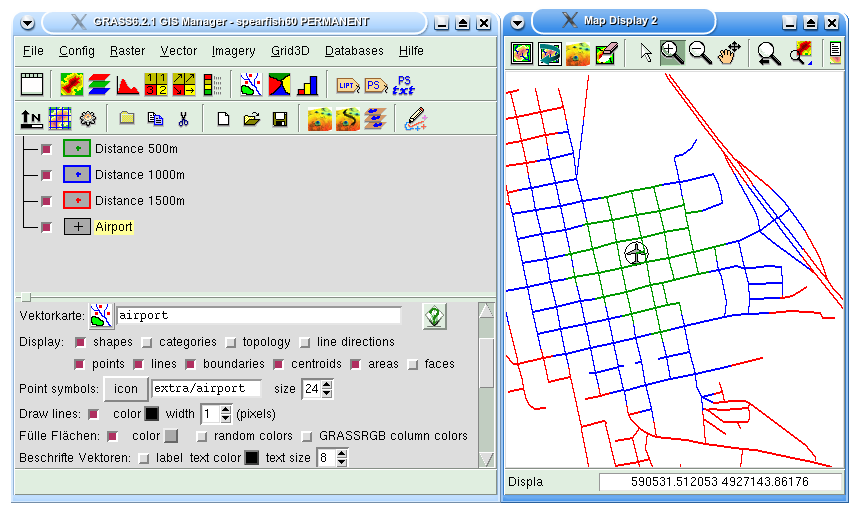
\includegraphics[width=0.7\textwidth]{isodist}
\captionof{figure}{Výchozí konfigurace GUI ukazující možnosti GRASSu pro síťové analýzy}
\end{myfig}

\subsection{Obrazové datové formáty}

CEOS (SAR, SRTM, LANDSAT7 etc.), ERDAS LAN / IMG, HDF, LANDSAT TM/MSS, NHAP aerial photos, SAR, SPOT, \dots
\begin{myfig}[1.5ex]
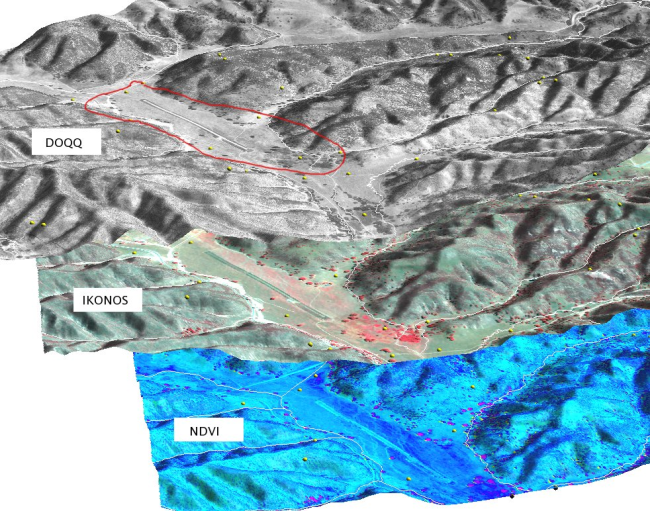
\includegraphics[width=0.7\textwidth]{ndvi}
\captionof{figure}{Možnosti GRASS ve zpracování obrazových dat}
\end{myfig}

\subsection{Podpora databazí}

\begin{itemize}
\item PostgreSQL / PostGIS
\item MySQL
\item SQLite
\item ODBC
\item DBF
\end{itemize}

\subsection{Výstup}

\begin{itemize}
\item Moduly pro tvorbu mapových výstupů
\item NVIZ pro vizualizaci 2.5D a 3D dat (tvorba animací \& pohledů)
%\item{GMT export}
%item{VRML}
\item VTK, POVray
\item WebGIS pomocí Mapserver, Python, a pod.
\end{itemize}

\subsection{Interoperabilita vůči dalším  GIS programům}

\begin{itemize}
\item Quantum GIS (Free Geodata (nejen) prohlížeč)
\item R- Language (statistika)
\item Gstat (geostatistika)
\item UMN Mapserver (webové služby)
\end{itemize}

\section{Kde najít další informace}

\begin{itemize}
%\begin{flushleft}
\item{Webové stránky projektu: \\\GRASSurl}
\item{GRASS Wiki: \\\url{http://grass.gdf.hannover.de/wiki}}
\item{Propagační tým GRASSu: \\\url{malte@perlomat.de}}
\item{Elektronické konference GRASSu: \\\url{http://grass.itc.it/community/support.php}}
%\end{flushleft}
\end{itemize}

\vfill
\section{OSGeo}

GRASS je zakládajícím projektem Open Source Geospatial Foundation, která si klade za cíl tvorbu vysoce kvalitního Open Source GIS software. Pro další informace navštivte domovskou stránku OSGeo:
\begin{center}

\includegraphics[width=0.8\textwidth]{OSGeo_CMYK}\\
\url{http://www.osgeo.org}
\end{center}

\end{document}
